\section{The Hierarchization Problem}
\label{sec:41problem}

Let $\sgset \subset \clint{0, 1}^d$ be a general (sparse) grid that
may be spatially adaptive, i.e.,
of the form $\sgset = \{\gp{\*l,\*i} \mid (\*l, \*i) \in \liset\}$,
where $\liset$ is a set of level-index pairs $(\*l, \*i)$ with $\*l \in \natz^d$
and $\*i \in \hiset{\*l}$ such that
$\ngp \ceq \setsize{\sgset} = \setsize{\liset} < \infty$
(see \cref{sec:233spatiallyAdaptiveSG}).
The \term{hierarchization problem} is finding
\term{hierarchical surpluses}
$(\surplus{\*l',\*i'})_{(\*l',\*i') \in \liset} \in \real^{\ngp}$ such that
\begin{equation}
  \label{eq:hierarchizationProblem}
  \largesum{(\*l', \*i') \in \liset} \surplus{\*l',\*i'}
  \basis{\*l',\*i'}(\gp{\*l,\*i}) = \fcnval{\*l,\*i}
  \quad\text{for all}\quad
  (\*l, \*i) \in \liset,
\end{equation}
where $\basis{\*l',\*i'}$ are arbitrary tensor product basis functions and
$(\fcnval{\*l,\*i})_{(\*l,\*i) \in \liset} \in \real^{\ngp}$ is a set of
function values $\objfun(\gp{\*l,\*i})$
at the grid points $\gp{\*l,\*i}$.
This then defines the interpolant $\sgintp$ as
\begin{equation}
  \label{eq:hierarchizationInterpolant}
  \sgintp\colon \clint{\*0, \*1} \to \real,\quad
  \sgintp \ceq
  \largesum{(\*l', \*i') \in \liset} \surplus{\*l',\*i'}
  \basis{\*l',\*i'},
\end{equation}
which interpolates $\objfun$ at the grid points $\gp{\*l,\*i}$ of $\sgset$.
\Cref{fig:hierarchization} shows the process of hierarchizing given
function values and evaluating the resulting interpolant.

\begin{figure}
  \subcaptionbox{%
    The objective function $\objfun$ is sampled at the grid points
    $\gp{l,i} \in \sgset$ to obtain function values $\fcnval{l,i}$,
    which form the input vector $\vlinin$ for the linear operator
    $\linop = \intpmatinv$.%
  }[46mm]{%
    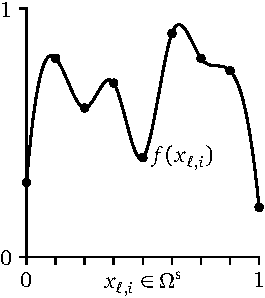
\includegraphics{hierarchization_1}%
  }%
  \hfill%
  \subcaptionbox{%
    The linear operator $\linop$ is applied to $\vlinin$ to obtain
    the output vector $\vlinout$, which contains the hierarchical surpluses
    $\surplus{l,i}$ ($(l,i) \in \liset$).%
  }[46mm]{%
    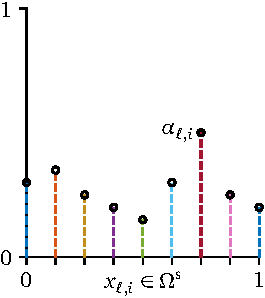
\includegraphics{hierarchization_2}%
  }%
  \hfill%
  \subcaptionbox{%
    The interpolant $\sgintp$ \emph{(black dashed line)}
    is evaluated at $x \in \clint{0, 1}$
    by adding contributions \emph{(black dotted lines)}
    of weighted basis functions $\surplus{l,i} \basis{l,i}$
    \emph{(colored),} obtaining $\sgintp(x)$ \emph{(cross).}%
  }[46mm]{%
    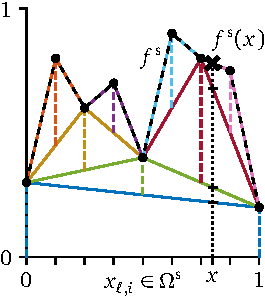
\includegraphics{hierarchization_3}%
  }%
  \caption[%
    Hierarchization of function values and evaluation of interpolant%
  ]{%
    Hierarchization of function values $\fcnval{l,i}$ \emph{(left)}
    to obtain hierarchical surpluses $\surplus{l,i}$ \emph{(center)} and
    evaluation of the resulting interpolant $\sgintp$ \emph{(right),}
    using a univariate grid and the piecewise linear basis as an example.%
  }%
  \label{fig:hierarchization}%
\end{figure}

We explicitly allow $\basis{\*l',\*i'}$ to be nodal basis functions,
in which case $\*l'$ is constant and
$\sgset$ is a full grid.
Strictly speaking, the problem is then an \term{interpolation problem}
and the $\surplus{\*l',\*i'}$ are \term{interpolation coefficients.}
However, we still apply the terms
``hierarchization'' and ``hierarchical surpluses'' in this case
to keep the terminology consistent.

\paragraph{Hierarchization as a linear operator}

The example of hierarchization can be generalized
to arbitrary linear operators
\begin{equation}
  \linop\colon \real^{\ngp} \to \real^{\ngp},\quad
  \vlinin \mapsto \vlinout = \linop[\vlinin],
\end{equation}
where $\linop$ depends on the grid $\sgset$ at hand.
Input $\vlinin$ and output $\vlinout$ are scalar-valued data%
\begin{equation}
  \vlinin = (\linin{\*l,\*i})_{(\*l,\*i) \in \liset} \in \real^{\ngp},\quad
  \vlinout = (\linout{\*l,\*i})_{(\*l,\*i) \in \liset} \in \real^{\ngp},
\end{equation}
which give one scalar per grid point $\gp{\*l,\*i} \in \sgset$.
For the case of hierarchization,
$\linop$ is the inverse of the \term{interpolation matrix}
$\intpmat \in \real^{\ngp \times \ngp}$:
\begin{subequations}
  \label{eq:hierarchizationSLE}
  \begin{equation}
    \linop = \intpmatinv,\quad
    \intpmat = (\basis{\*l',\*i'}(\gp{\*l,\*i}))_%
    {(\*l,\*i),(\*l',\*i') \in \liset},\quad
    \vlinin = (\fcnval{\*l,\*i})_{(\*l,\*i) \in \liset},\quad
    \vlinout = (\surplus{\*l',\*i'})_{(\*l',\*i') \in \liset}.
    \hspace*{-1mm}
  \end{equation}
  This means that we can determine the $\surplus{\*l',\*i'}$ by solving
  the $\ngp \times \ngp$ system of linear equations
  \begin{equation}
    \vlinout = \linop[\vlinin]
    \quad\iff\quad
    \intpmat \cdot (\surplus{\*l',\*i'})_{(\*l',\*i') \in \liset}
    = (\fcnval{\*l,\*i})_{(\*l,\*i) \in \liset}.
  \end{equation}
\end{subequations}

\paragraph{Complexity of B-spline hierarchization}

As noted in \cite{Valentin18Fundamental},
hierarchization on sparse grids with hierarchical B-splines
$\bspl{\*l,\*i}{\*p}$ of degree $\*p$
as basis functions $\basis{\*l,\*i}$ is a tedious task.
The corresponding linear system \eqref{eq:hierarchizationSLE} is in general
non-symmetric
(i.e., $\bspl{\*l',\*i'}{\*p}(\gp{\*l,\*i}) \not=
\bspl{\*l,\*i}{\*p}(\gp{\*l',\*i'})$) and densely populated.
This is because the matrix entry in the $(\*l,\*i)$-th row and
$(\*l',\*i')$-th column vanishes if and only if
\begin{equation}
  \gp{\*l,\*i} \notin \interiorsupp \bspl{\*l',\*i'}{\*p}
  \iff
  \exlarge{t = 1, \dotsc, d}{
    \gp{l_t,i_t} \notin
    \opintscaled{
      \gp{l'_t,i'_t} - \tfrac{p_t+1}{2} \ms{l'_t},\,
      \gp{l'_t,i'_t} + \tfrac{p_t+1}{2} \ms{l'_t}
    }
  },
\end{equation}
where $\interiorsupp$ is the interior of the support
\cite{Valentin18Fundamental}.
For coarse levels $\*l'$, the mesh size $\ms{l'_t}$ is large in
every dimension $t$, which implies that $\interiorsupp \bspl{\*l',\*i'}{\*p}$
contains most of the grid points.
In contrast to the hat function case ($\*p = \*1$),
the value of $\surplus{\*l',\*i'}$ depends not only on
$\fcnval{\*l,\*i}$ and the data of the $3^d - 1$ neighboring grid points
on the boundary of $\supp \bspl{\*l',\*i'}{\*1}$,
but potentially on the data of the whole grid.
This is shown in \cref{fig:matrixDensityPattern}:
There are at most $3^d = 9$ non-zero entries in each row of $\intpmatinv$
for $\*p = \*1$ and $d = 2$.
As soon as the B-spline degree is increased,
both $\intpmat$ and $\intpmatinv$ become significantly denser.

\begin{SCfigure}
  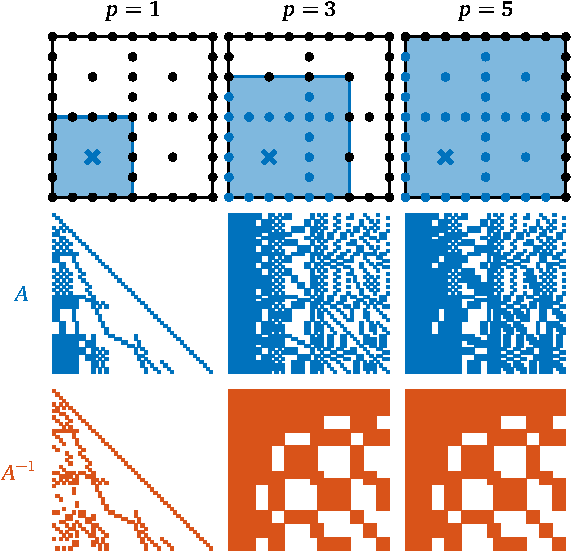
\includegraphics{matrixDensityPattern_1}%
  \caption[%
    Density pattern of hierarchization matrices and of their inverses%
  ]{%
    Density pattern
    of the hierarchization matrix $\intpmat$
    \emph{(middle row, \textcolor{C0}{blue})} and
    of its inverse $\intpmatinv$
    \emph{(bottom row, \textcolor{C1}{red})}
    for the regular sparse grid $\coarseregsgset{n}{d}{1}$
    with $n = 4$ and $d = 2$ \emph{(top row)}
    and uniform hierarchical B-splines $\bspl{\*l,\*i}{\*p}$
    for degrees $\*p \in \{\*1, \*3, \*5\}$.
    The \textcolor{C0}{blue areas} in the top row
    show the extent of the support of one specific basis function
    $\bspl{\*l',\*i'}{\*p}$ with $\*l' = (2, 2)$ and $\*i' = (1, 1)$
    (\emph{cross:} corresponding grid point $\gp{\*l',\*i'}$).
    The \textcolor{C0}{blue points} are the grid points at which
    $\bspl{\*l',\*i'}{\*p}$ is non-zero.%
  }%
  \label{fig:matrixDensityPattern}%
\end{SCfigure}

This prohibits the use of the \up\punctfix{,}
which we will discuss in the next section,
on sparse grids with hierarchical B-splines.
Consequently, we have to solve the linear system
\eqref{eq:hierarchizationSLE}, which is significantly more time-consuming,
as it takes between $\landauOmega{\ngp^2 d}$ and $\landauO{\ngp^2 (N+d)}$ time
via Gaussian elimination.%
\footnote{%
  $\landauOmega{\ngp^2 d}$ for assembling $\intpmat$ and
  $\landauO{\ngp^3}$ for solving the system.
}
In addition, if we use an explicit solver for the linear system,
we additionally have to store an $\ngp \times \ngp$ matrix in memory.
However, a grid of size $\ngp = \num{116000}$ already exceeds the memory
of a \SI{128}{\gibi\byte} supercomputer node,
if we explicitly store the full matrix in double precision.
In comparison, for the hat function basis,
the \up only requires $\landauO{\ngp d}$ time and $\landauO{\ngp}$ memory.

\paragraph{Notation}

We do not need the hierarchical level-index information $(\*l, \*i)$ in
$\sgset$, $\liset$, $\vlinin$, and $\vlinout$
for most of the considerations in this chapter.
In these cases, we assume that in each dimension $t$, the level-index pairs
$(l_t, i_t)$ ($l_t \in \natz$, $i_t \in \hiset{l_t}$)
are continuously enumerated by a single index $k_t = k_t(l_t, i_t) \in \natz$.
We identify $(\*l, \*i)$ with a single index $\*k$,
whose $t$-th component is given by $k_t(l_t, i_t)$.
Hence,
we regard $\liset$ as a subset $\liset \ceq \{\*k \mid \*x_\*k \in \sgset\}$
of $\natz^d$.
We will switch between the notations whenever appropriate.
All statements that are formulated in the $\*k$ notation are
valid for both the nodal and the hierarchical basis.

\usenotation{kT00}
In the following, $k_t$ denotes the $t$-th component of a $d$-vector $\*k$
as usual.
\usenotation{kT10}
With $\*k_{-t}$, we denote the $(d-1)$-vector that is obtained from $\*k$
by omitting the $t$-th component,
i.e., $\*k_{-t} \ceq (k_1, \dotsc, k_{t-1}, k_{t+1}, \dotsc, k_d)$.
\usenotation{kT20}
For a $j$-tuple $T = (t_1, \dotsc, t_j) \in \{1, \dotsc, d\}^j$,
we define $\*k_T$ to be the $j$-vector $(k_{t_1}, \dotsc, k_{t_j})$
that only contains the entries of the dimensions listed in $T$.
\usenotation{kT30}
Accordingly, $\*k_{-T}$ is defined as the $(d-j)$-vector
that contains the entries of the remaining dimensions
(sorted by the dimension $t$).
We define $\*k_{\range{a}{b}} \ceq (k_a, k_{a+1}, \dotsc, k_b)$
as an indexing shortcut ($a \le b$).
